% !TEX root = main.tex
\documentclass[11pt,xcolor={dvipsnames},hyperref={pdftex,pdfpagemode=UseNone,hidelinks,pdfdisplaydoctitle=true},usepdftitle=false]{beamer}
\usepackage{../include/presentation}
\usepackage{tikz}
\title{Multi-Robot Waypoint Inspection Plan Mixed Integer Linear Programming Project}
\author{Juan Carlos Cruz - ira406}
\date{ME 6033 Linear and Mixed Integer Optimization}
\begin{document}
    
    \begin{frame}
      \titlepage
      April 2025
    \end{frame}
    
    \begin{frame}{Introduction}
      \begin{itemize}
        \item Based on previous work done in an outdoor concrete inspection multirobot framework
        \item Precast concrete elements require efficient inspection methods after being transported to a site
        \item Multi-robot approach:
          \begin{itemize}
            \item Aerial robots locate targets
            \item Ground robots perform detailed inspections
          \end{itemize}
        \item For this project wanted to see if we could extend this idea to planning of multiple robots across an inspection site
      \end{itemize}

      \begin{figure}
        \centering
        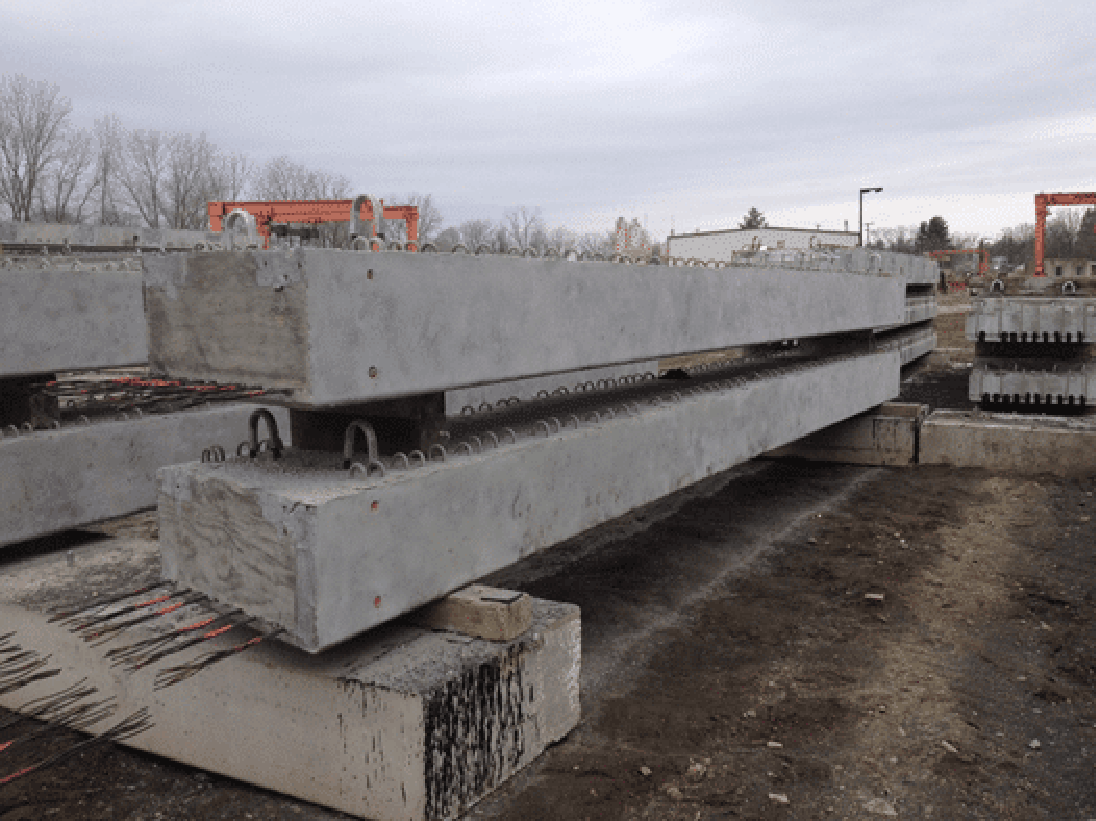
\includegraphics[width=0.3\linewidth]{figures/concrete.pdf}
        \caption{\tiny{\url{https://kta.com/inspection-of-the-precast-prestressed-concrete-fabrication-process/}}}
      \end{figure}
    \end{frame}

    \begin{frame}{Problem Description}
      \begin{itemize}
        \item Two robot types: aerial and ground mobile robots
        \item Inspection targets as waypoints in a 2D plane
        \item Depot location for each robot type
        \item Sequential operation:
          \begin{itemize}
            \item Aerial robots verify waypoint location first
            \item Ground robots perform detailed inspection second
          \end{itemize}
        \item Robot constraints:
          \begin{itemize}
            \item Fixed speeds (meters/minute)
            \item Limited operation time (battery life time after leaving depot)
            \item Required inspection time at waypoints
          \end{itemize}
        \item Objective: Maximize waypoint visits in a single inspection loop. 
        \item Becomes a MILP problem. Linear objective function and linear constraints but use binary and continuous variables. 
      \end{itemize}

    \end{frame}

    \begin{frame}{Literature Review}
      \begin{itemize}
        \item Prior works demonstrate multi-robot planning applications
        \item Problem resembles multiple traveling salesman problem (mTSP)
        \item Traditional MILP for mTSP:
          \begin{itemize}
            \item Routing variables 
            \item Subtour elimination constraints
          \end{itemize}
        \item Initially tried this approach but solving time was too slow and larger problems became infeasible (likely implementation error) so used a simplification
        \item Route approximation: roundtrip distances from depot to waypoints estimate travel times
      \end{itemize}
    \end{frame}

    \begin{frame}{Model}
      \begin{figure}
        \begin{minipage}{0.5\textwidth}
          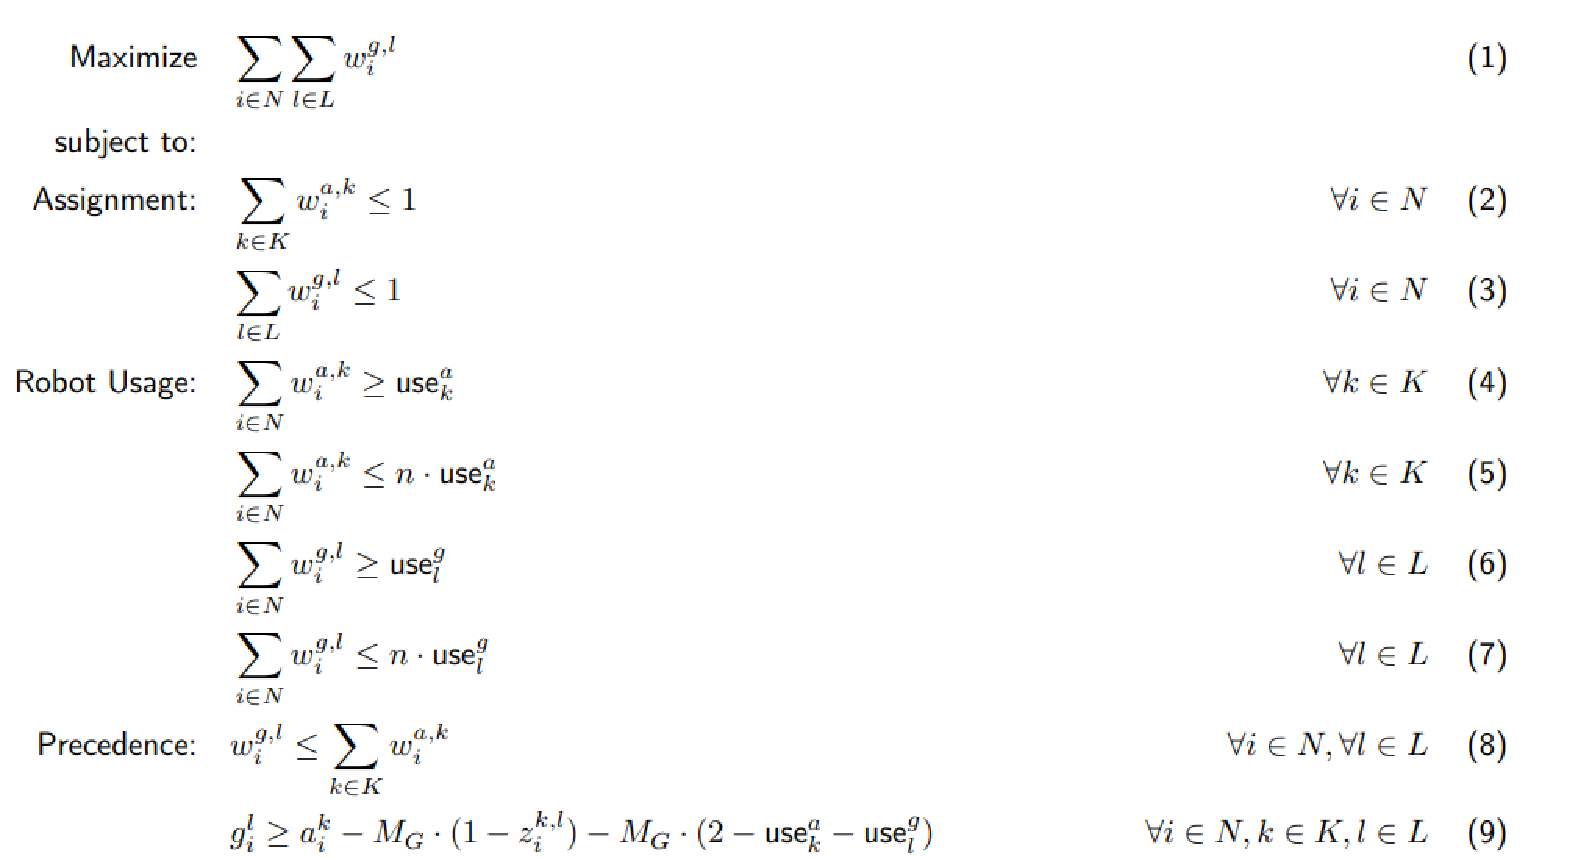
\includegraphics[width=\textwidth]{figures/opt1.pdf}
        \end{minipage}
        \hfill
        \begin{minipage}{0.5\textwidth}
          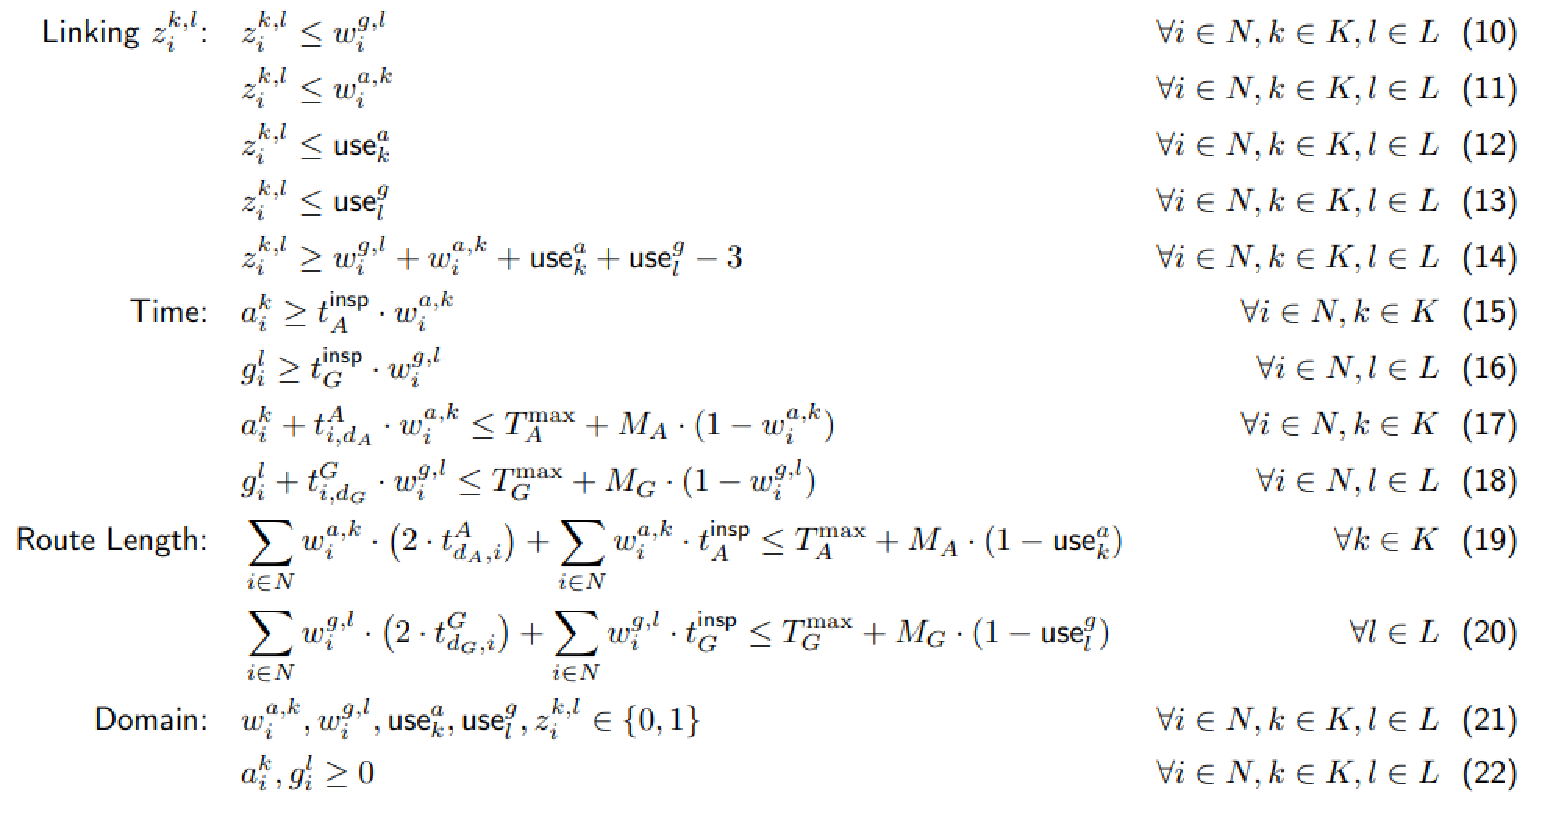
\includegraphics[width=\textwidth]{figures/opt2.pdf}
        \end{minipage}
      \end{figure}
    \end{frame}

  \begin{frame}{Solution Method}
    \begin{itemize}
      \item Implemented in Python using PuLP library
      \item CBC solver from PuLP used for optimization
      \item Interactive browser-based GUI developed:
        \begin{itemize}
          \item Parameter input for robot specifications
          \item Waypoint location setting
          \item Real-time solution visualization
        \end{itemize}
      \item Code available at \href{https://github.com/jc-cr/multirobot_inspection_optimizer}{GitHub repository}
    \end{itemize}
    
        % Insert demo image
        \begin{figure}
          \centering
          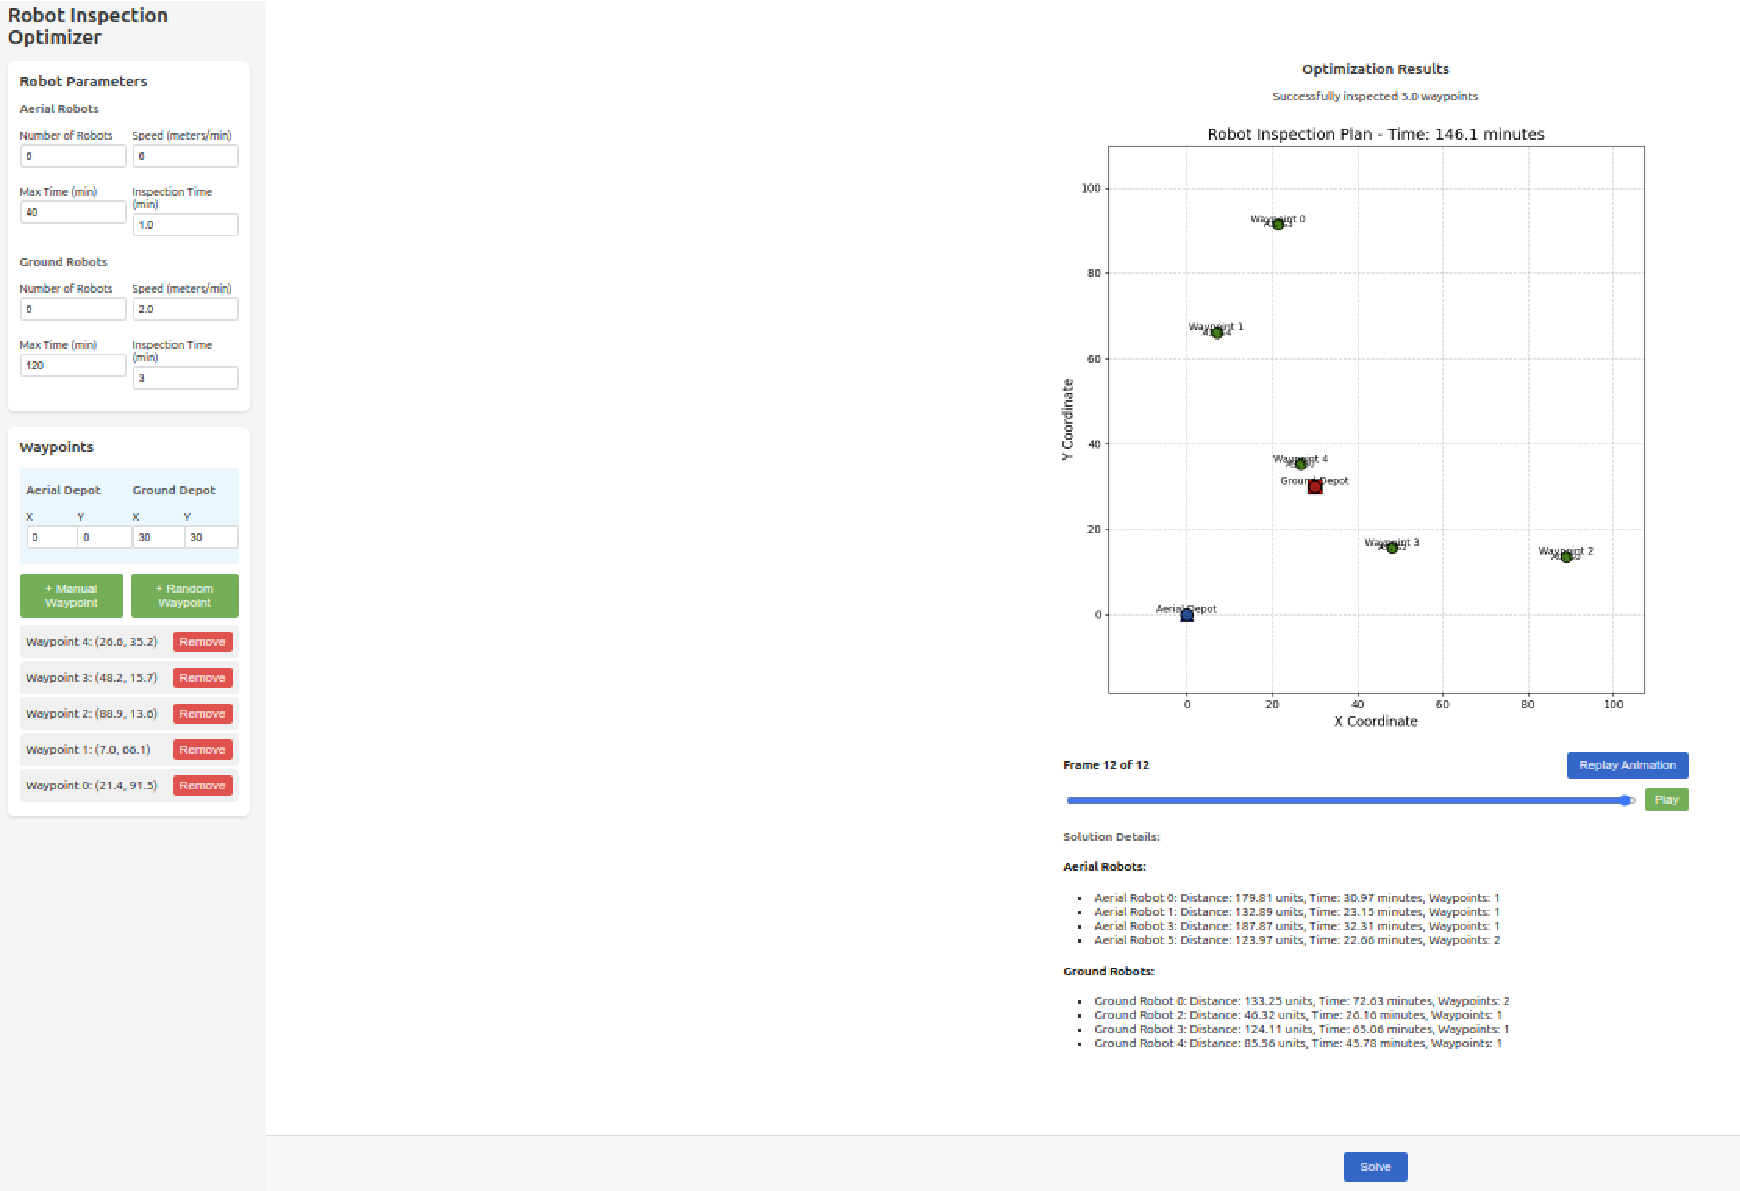
\includegraphics[width=0.5\linewidth]{figures/insp.pdf}
        \end{figure}
      \end{frame}

      \begin{frame}{Numerical Results - Computational Performance}
        \begin{itemize}
          \item Testing environment: 
            \begin{itemize}
            \item Intel i7, Python 3.12 Docker container
          \end{itemize}
        \item Tested waypoint scaling (5 to 25 waypoints) and map size scaling (100 to 1000 m)
        \item Non-monotonic scaling behavior:
          \begin{itemize}
            \item Solution time peaks at 15 waypoints then decreases
            \item Computation time peaks at 500m map size
          \end{itemize}
      \end{itemize}
      
      % Insert performance figures
      \begin{figure}
        \centering
        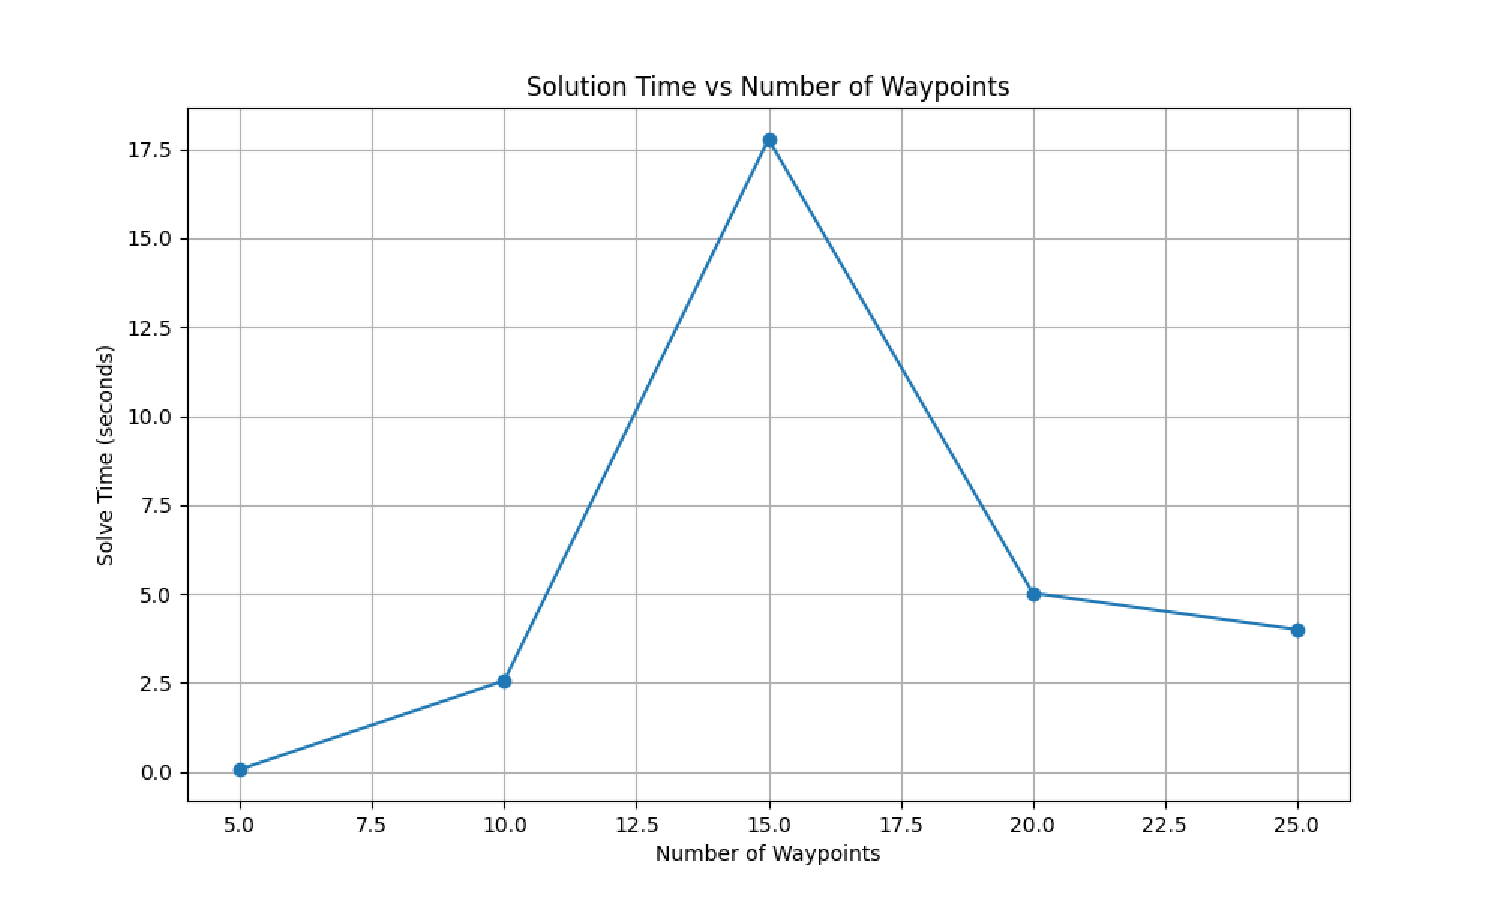
\includegraphics[width=0.48\linewidth]{figures/waypoints_vs_time.pdf}
        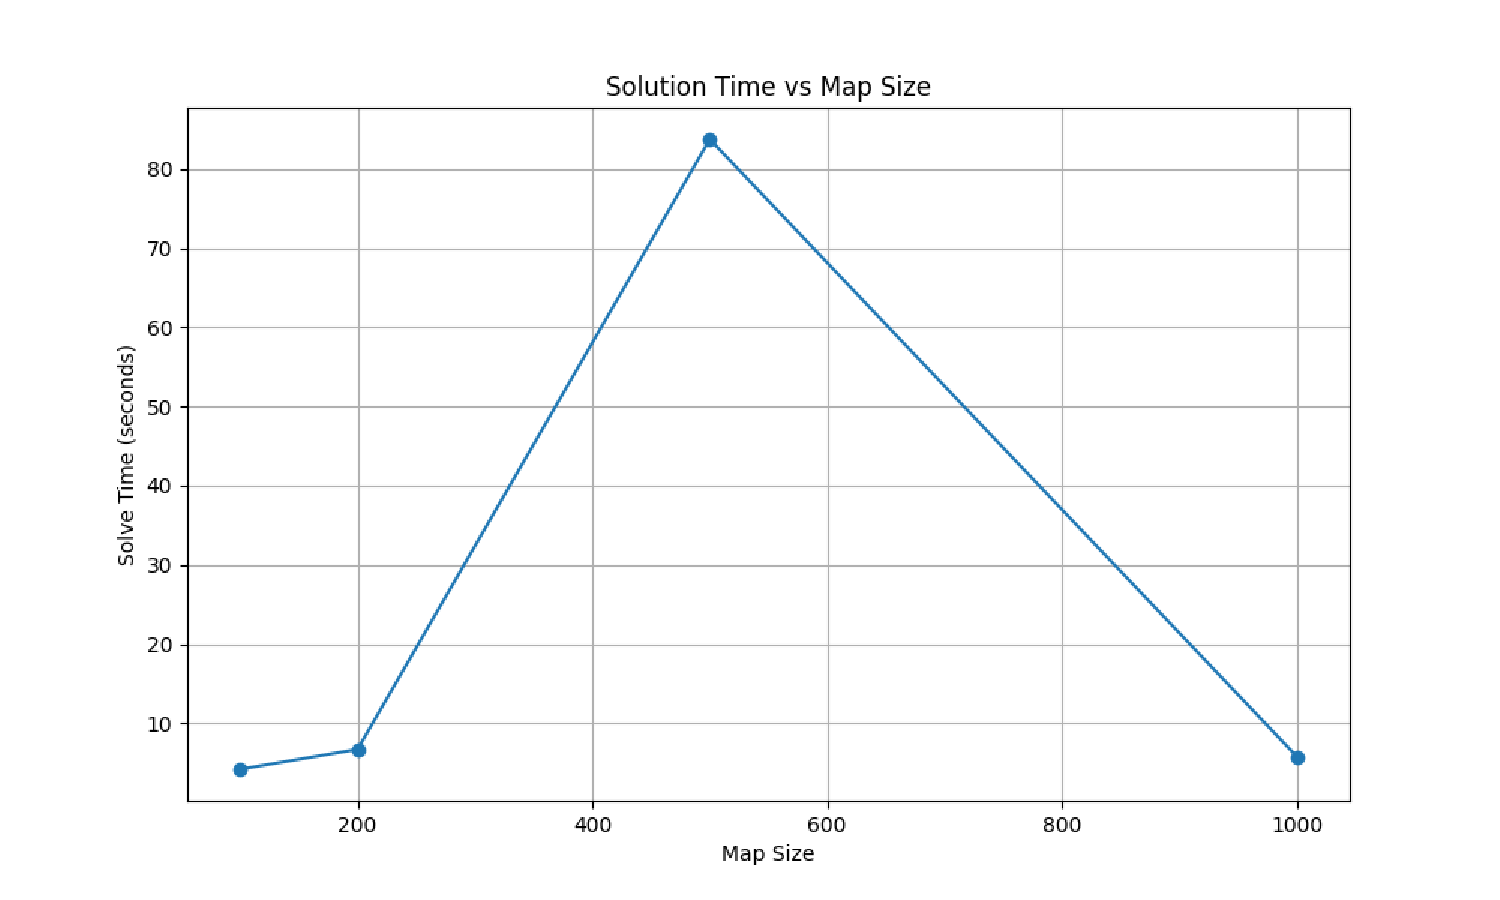
\includegraphics[width=0.48\linewidth]{figures/map_size_vs_time.pdf}
      \end{figure}
    \end{frame}

    \begin{frame}{Numerical Results - Sensitivity Analysis}
    \begin{columns}
      \begin{column}{0.48\textwidth}
        \begin{itemize}
          \item Using fixed waypoints and map size we solve multiple times varying 8 params: robot speeds, operation times, inspection times, and fleet sizes.
          \item Most influential parameters:
            \begin{itemize}
              \item Number of ground robots
              \item Aerial robot maximum operation time
            \end{itemize}
          \item Minimal impact: Inspection times
        \end{itemize}
      \end{column}
      
      \begin{column}{0.48\textwidth}
        \begin{figure}
          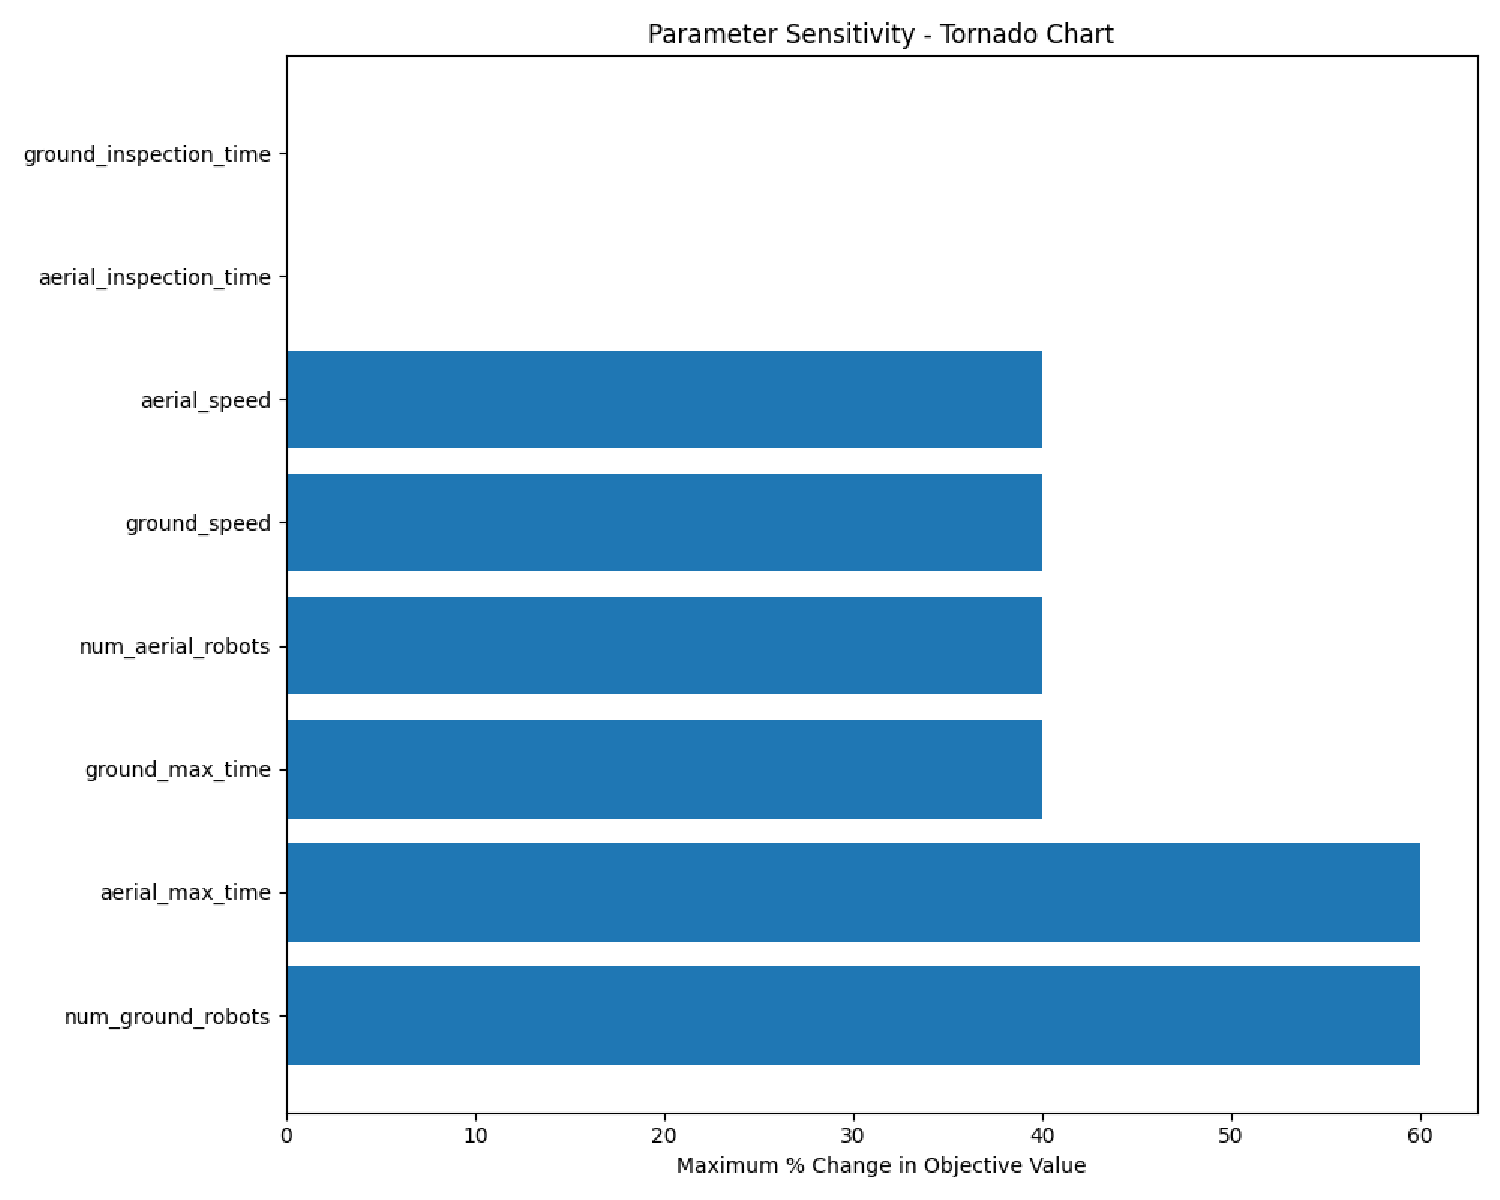
\includegraphics[width=\textwidth]{figures/tornado_chart.pdf}
        \end{figure}
      \end{column}
    \end{columns}
  \end{frame}

  \begin{frame}{Numerical Results - Ground Robot Sensitivity Analysis}
    \begin{columns}
      \begin{column}{0.46\textwidth}
        \begin{figure}
          \centering
          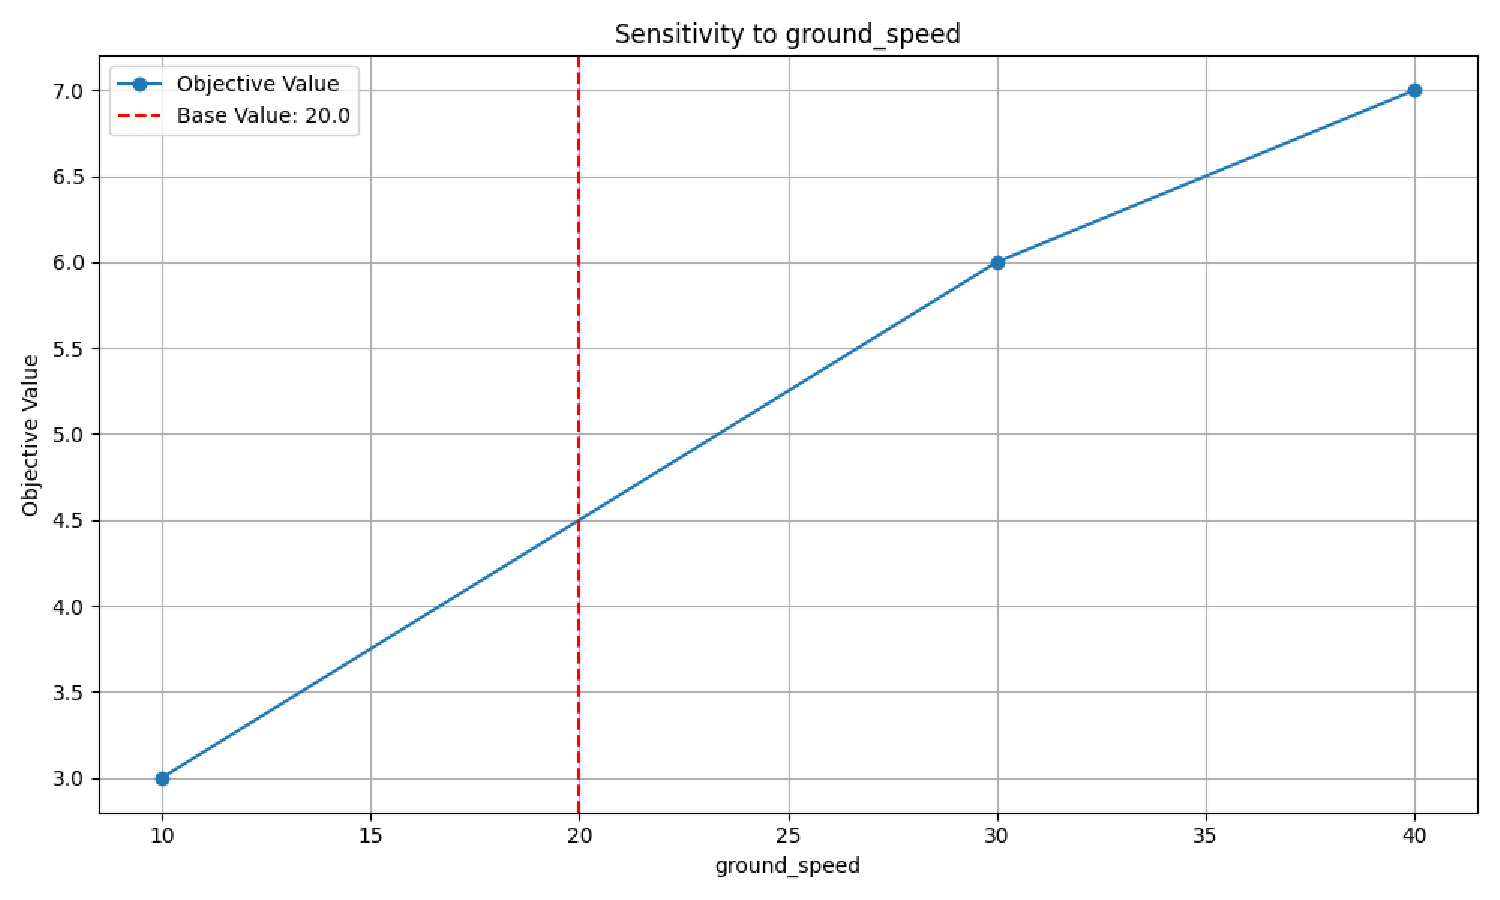
\includegraphics[width=\textwidth]{figures/sensitivity_ground_speed.pdf}
        \end{figure}
      \end{column}
      
      \begin{column}{0.46\textwidth}
        \begin{figure}
          \centering
          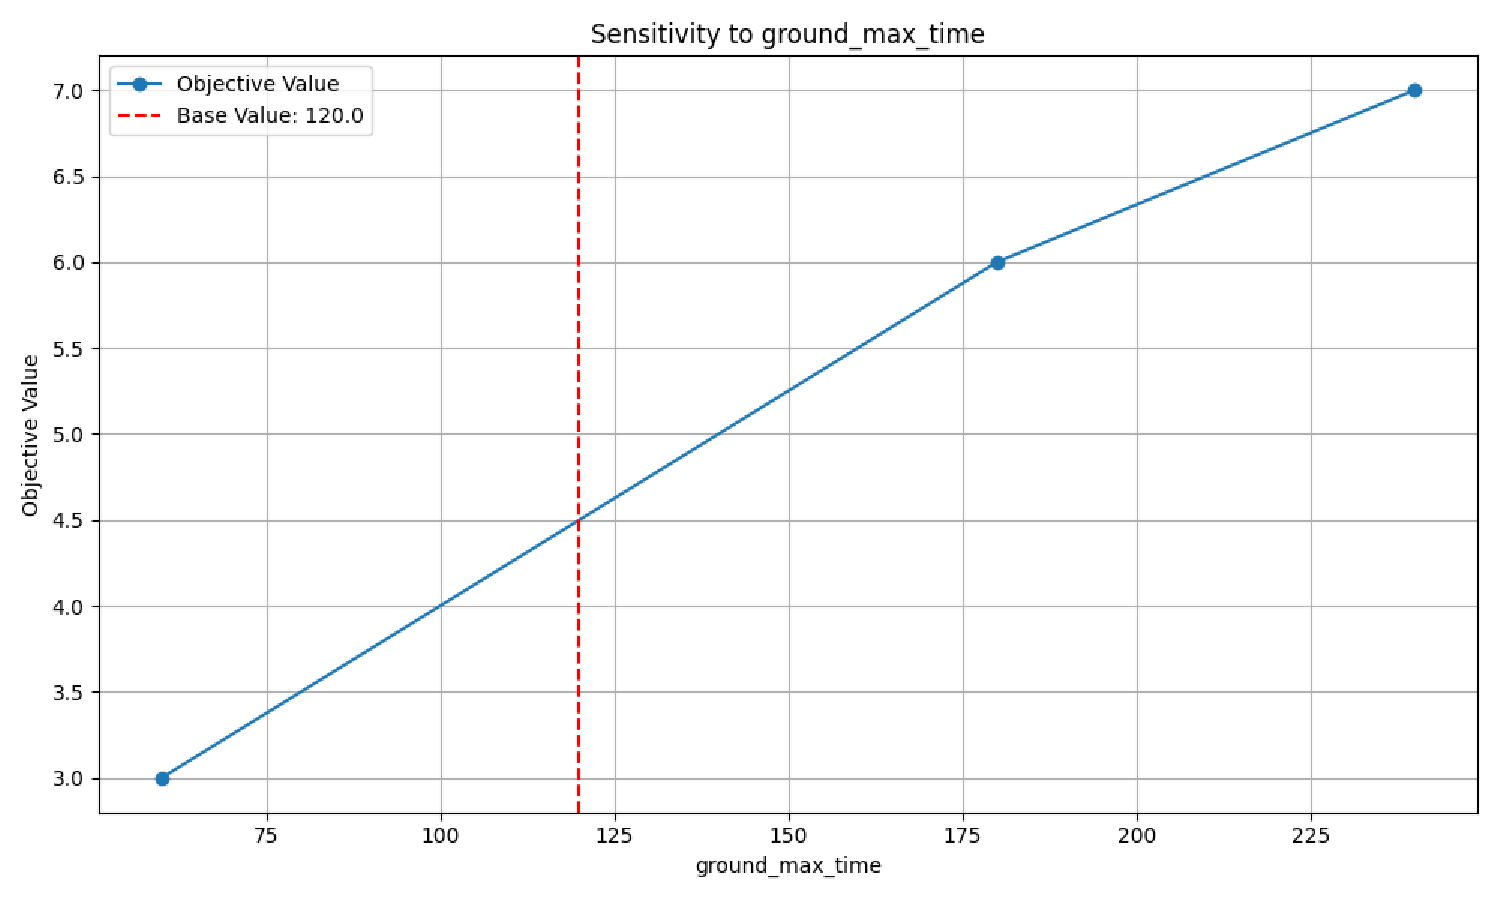
\includegraphics[width=\textwidth]{figures/sensitivity_ground_max_time.pdf}
        \end{figure}
      \end{column}
    \end{columns}
    
    
    \begin{columns}
      \begin{column}{0.46\textwidth}
        \begin{figure}
          \centering
          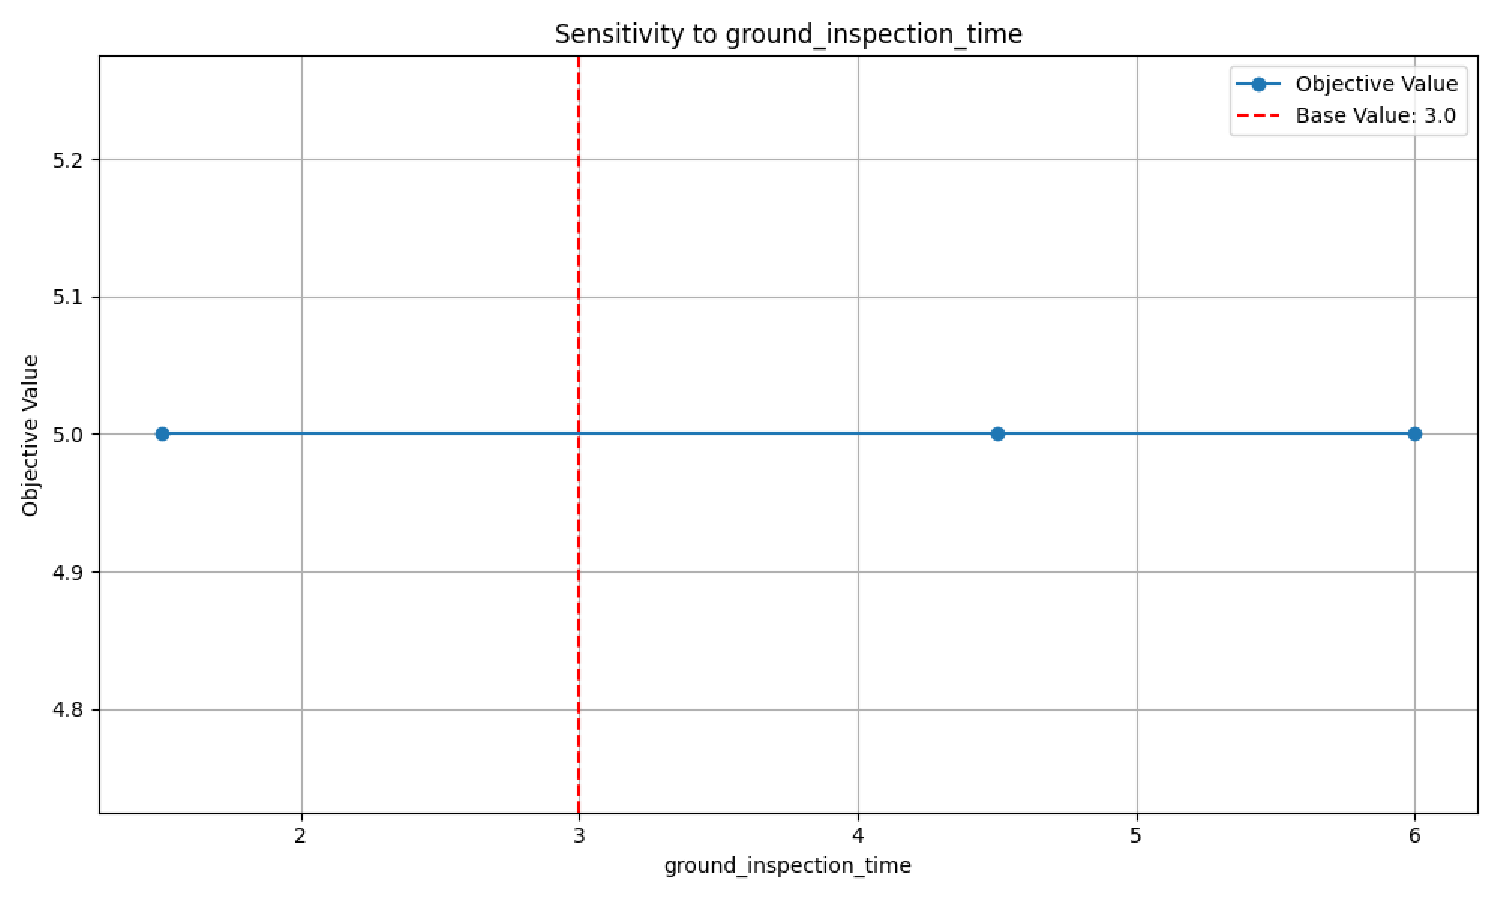
\includegraphics[width=\textwidth]{figures/sensitivity_ground_inspection_time.pdf}
        \end{figure}
      \end{column}
      
      \begin{column}{0.46\textwidth}
        \begin{figure}
          \centering
          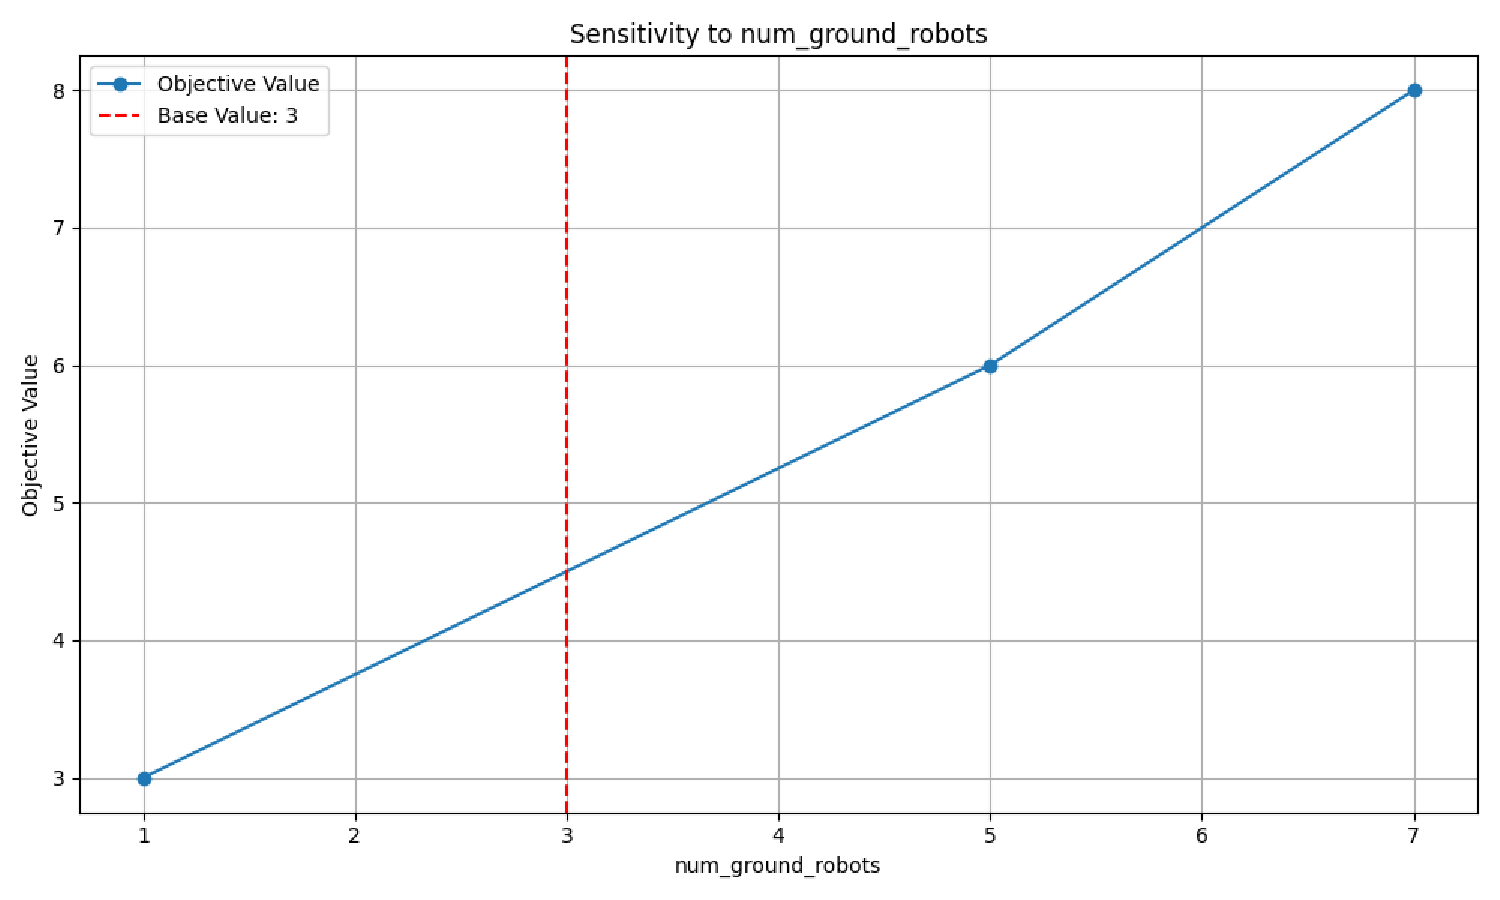
\includegraphics[width=\textwidth]{figures/sensitivity_num_ground_robots.pdf}
        \end{figure}
      \end{column}
    \end{columns}
  \end{frame}

\begin{frame}{Numerical Results - Aerial Robot Sensitivity Analysis}
  \begin{columns}
    \begin{column}{0.46\textwidth}
      \begin{figure}
        \centering
        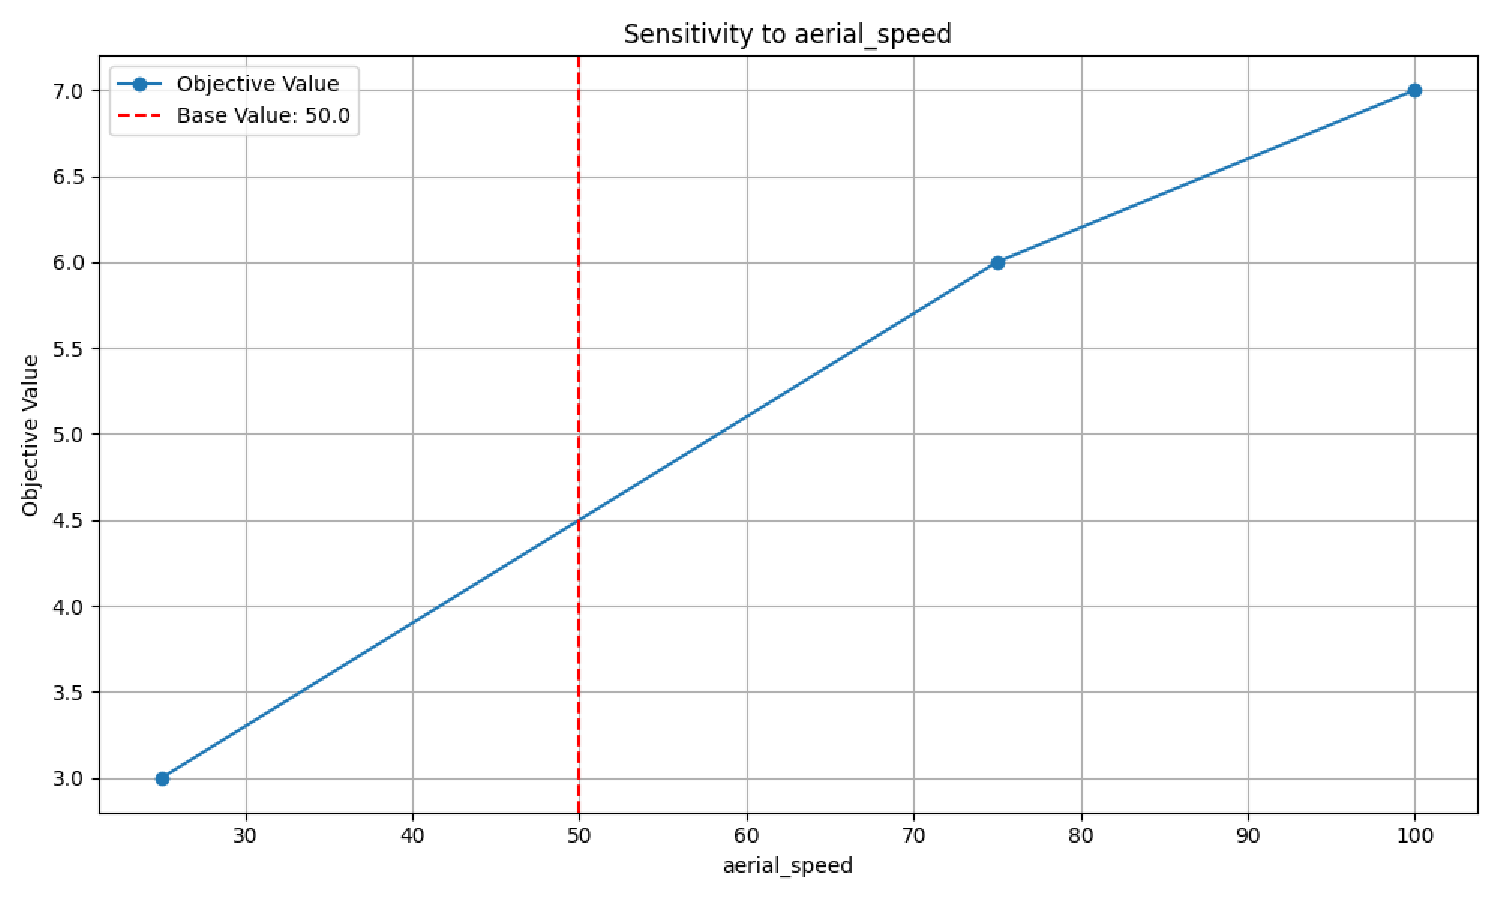
\includegraphics[width=\textwidth]{figures/sensitivity_aerial_speed.pdf}
      \end{figure}
    \end{column}
    
    \begin{column}{0.46\textwidth}
      \begin{figure}
        \centering
        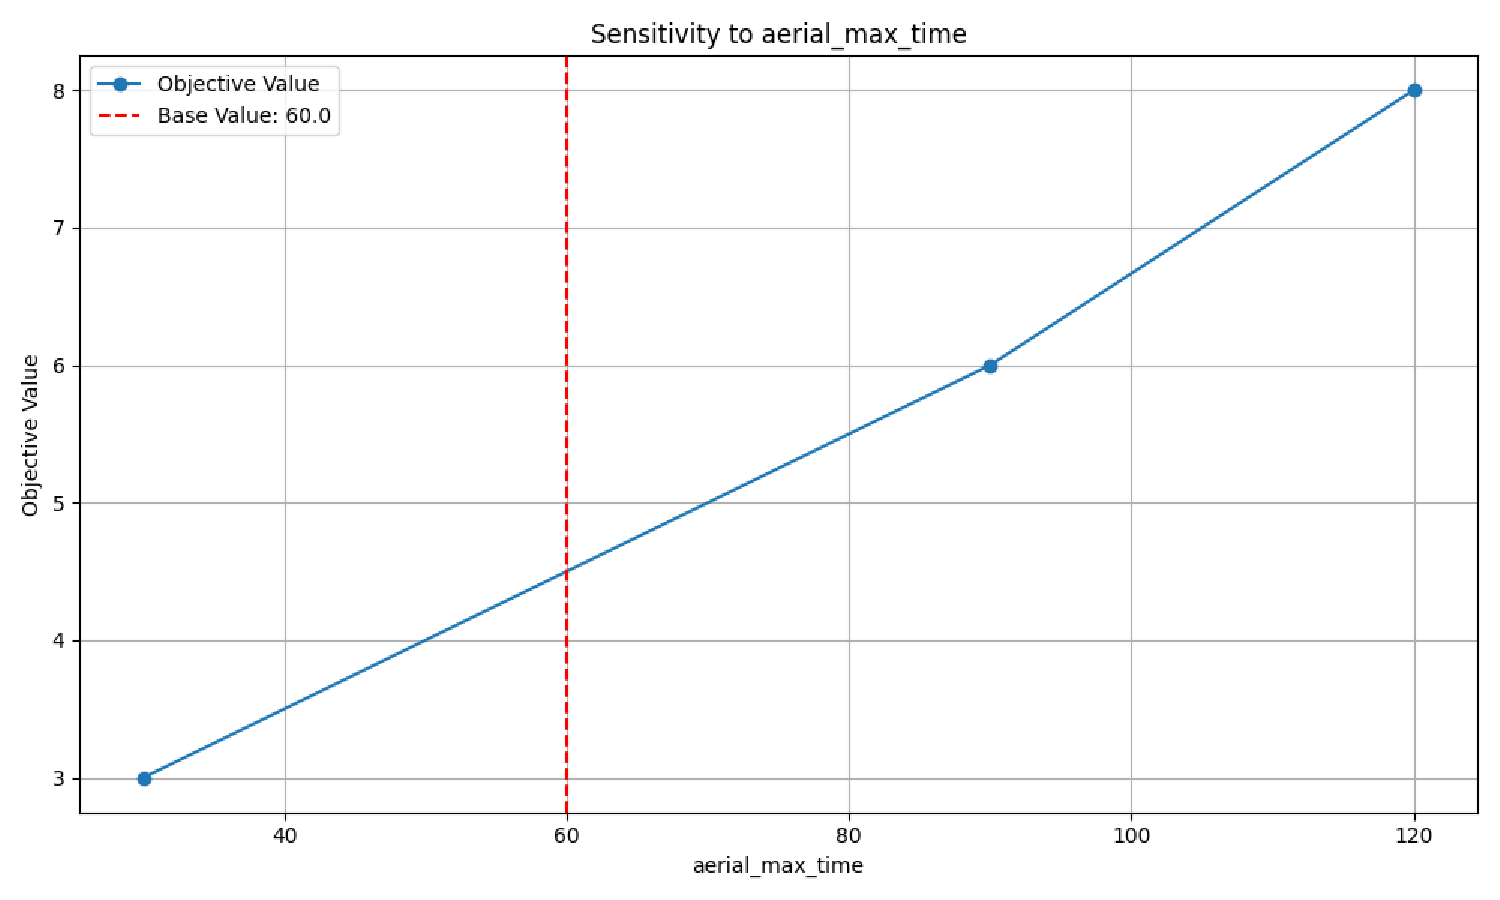
\includegraphics[width=\textwidth]{figures/sensitivity_aerial_max_time.pdf}
      \end{figure}
    \end{column}
  \end{columns}
  
  
  \begin{columns}
    \begin{column}{0.46\textwidth}
      \begin{figure}
        \centering
        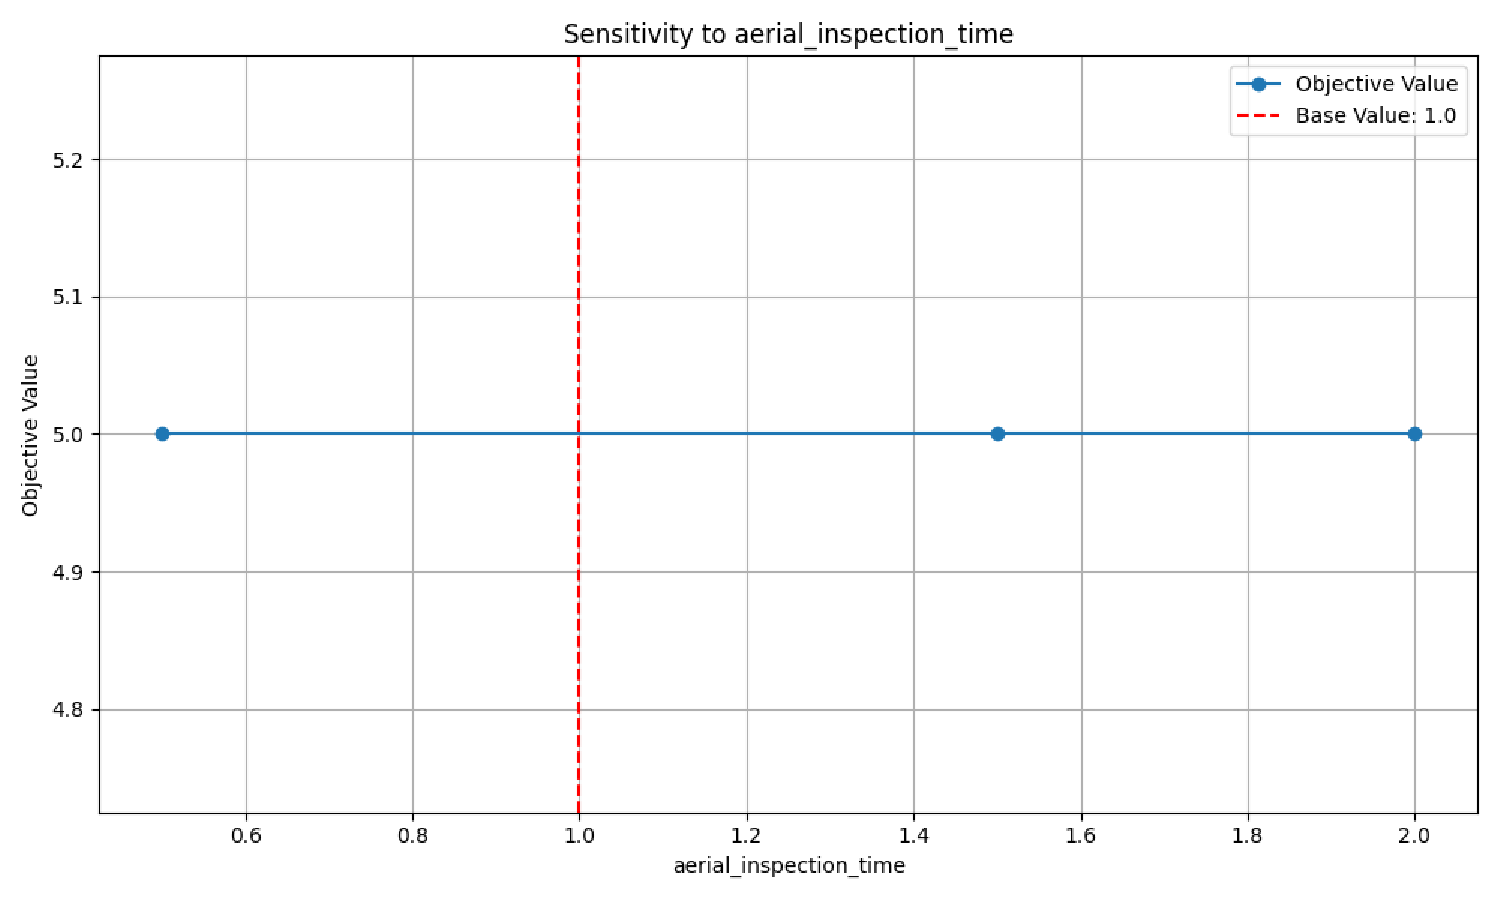
\includegraphics[width=\textwidth]{figures/sensitivity_aerial_inspection_time.pdf}
      \end{figure}
    \end{column}
    
    \begin{column}{0.46\textwidth}
      \begin{figure}
        \centering
        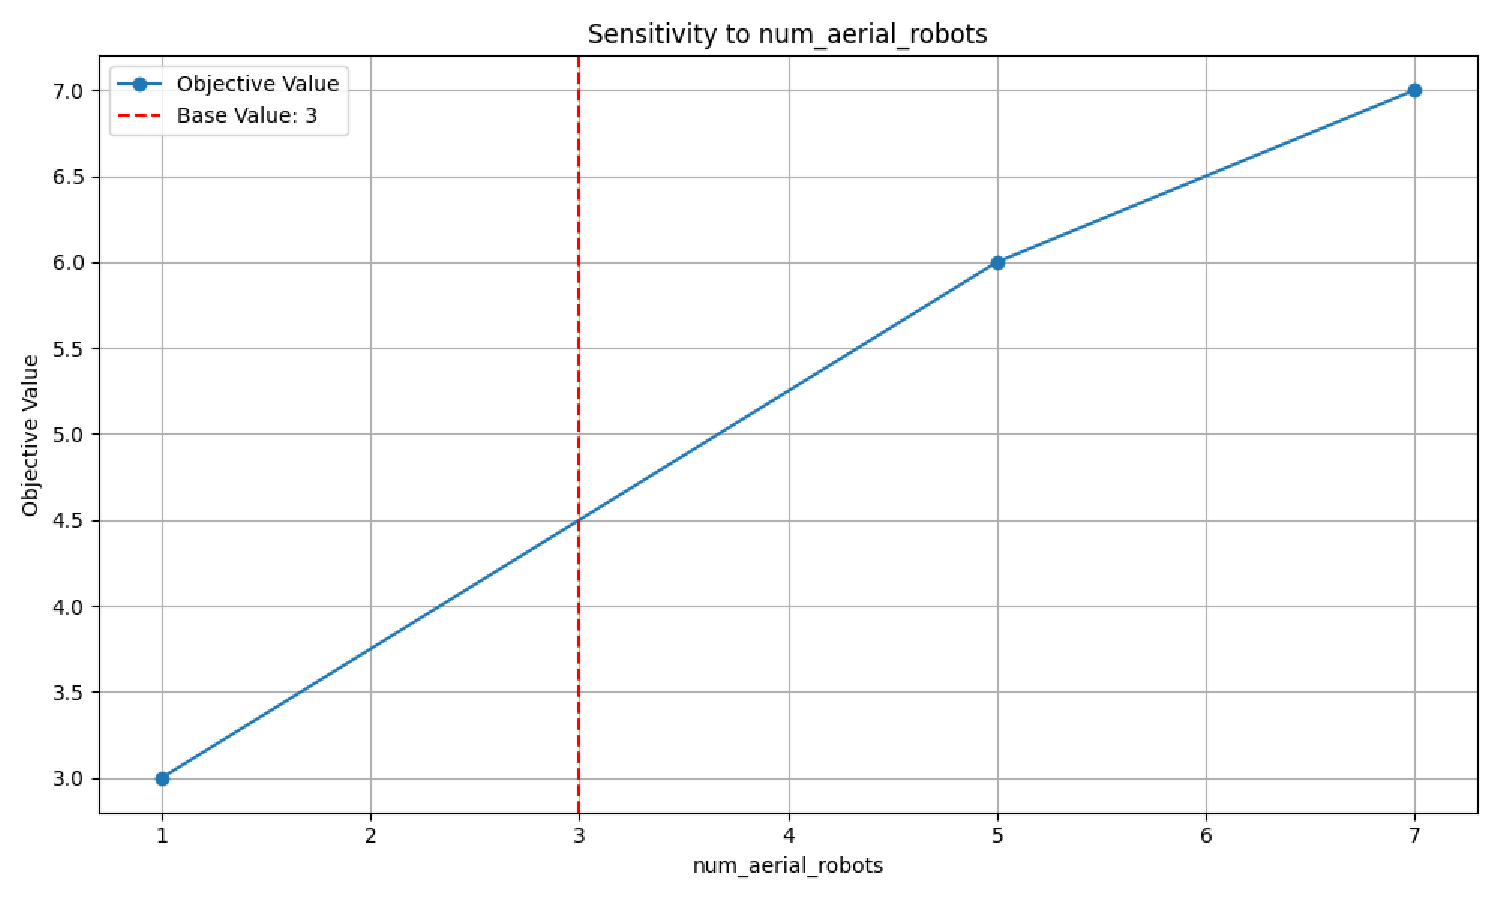
\includegraphics[width=\textwidth]{figures/sensitivity_num_aerial_robots.pdf}
      \end{figure}
    \end{column}
  \end{columns}
\end{frame}



  
    \begin{frame}{Demo Video}
    \centering
    \begin{figure}
      \centering
      \href{https://www.youtube-nocookie.com/embed/rC7g-lJ-lPA?playlist=rC7g-lJ-lPA&autoplay=1&iv_load_policy=3&loop=1&start=}{
        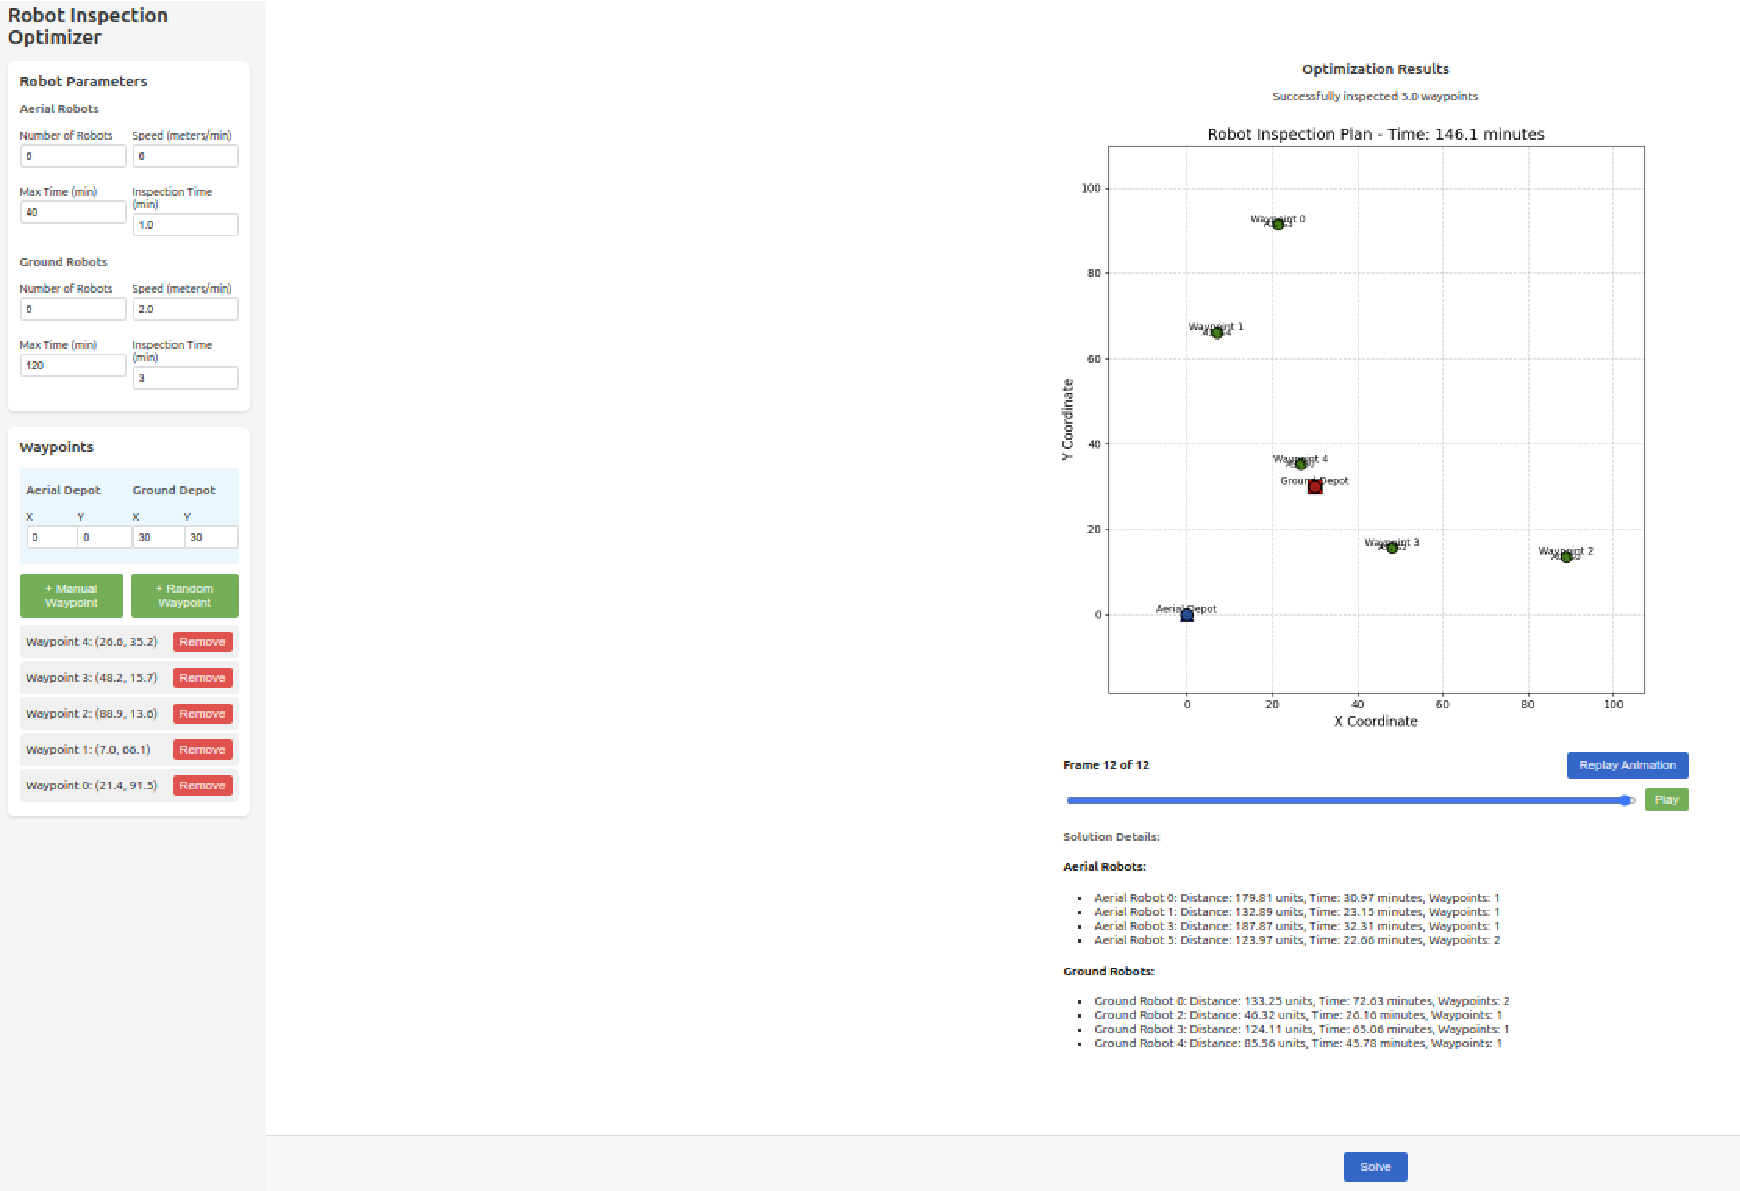
\includegraphics[width=0.7\linewidth]{figures/insp.pdf}
      }
      \caption{Click to watch the demo video}
    \end{figure}
  \end{frame}
    
    \lastslide
\end{document}